\section{Results and Discussion}
\subsection{2013 Results}
As it has already been pointed out, outlier channels from Figure~\ref{fig:QIE_Slope} have been excluded.
Moreover, to achieve a result for the average energy deposition per channel type,
EM or H, from the radioactive source, we only considered data from towers with
IEta $<$ 35 to minimize the effects from PMT gain drift, as observed in 2011 and
2012, shown in Figure~\ref{fig:PMT_Drift}.

\begin{figure}[htb]
   \begin{center}
      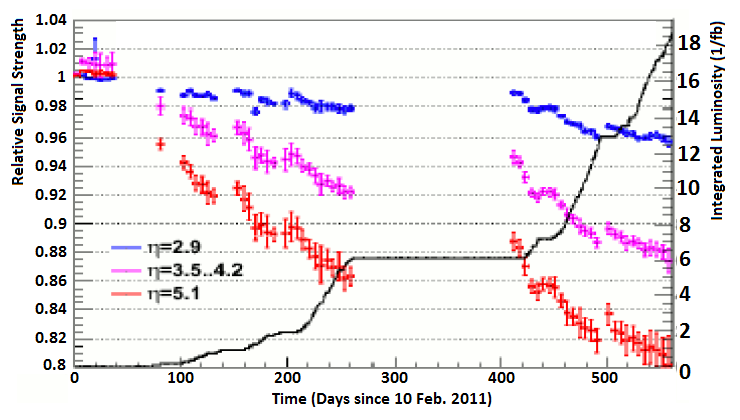
\includegraphics[width=.75\textwidth]{figures/ch_hfcalibration/PMT_Drift.png}
      \caption{R7525 PMT relative signal strength with respect to 10 Feb. 2011 as a
      function of time since that date, for various $\eta$ locations. The solid
      black curve represents the integrated luminosity within CMS over the same
      time period.}
      \label{fig:PMT_Drift}
   \end{center}
\end{figure}

Figure~\ref{fig:HFM_2013_Res} shows the results from 2013 when only the near side
of HF- was sourced, nine wedges, and only the towers below IEta = 35 are
considered, eight towers per wedge. The average energy deposition extracted from
2013 sourcing campaign, for EM and HAD channels separately, is 744.6 $\pm$ 6.3\unit{keV}/25\unit{ns} and 706.8 $\pm$ 7.7\unit{keV}/25\unit{ns}, respectively. There is a 5\% difference observed between the EM and HAD channels, while their
respective precision is kept within 1\% each.
\begin{figure}[!h]
   \begin{center}
      \subfigure[]{
         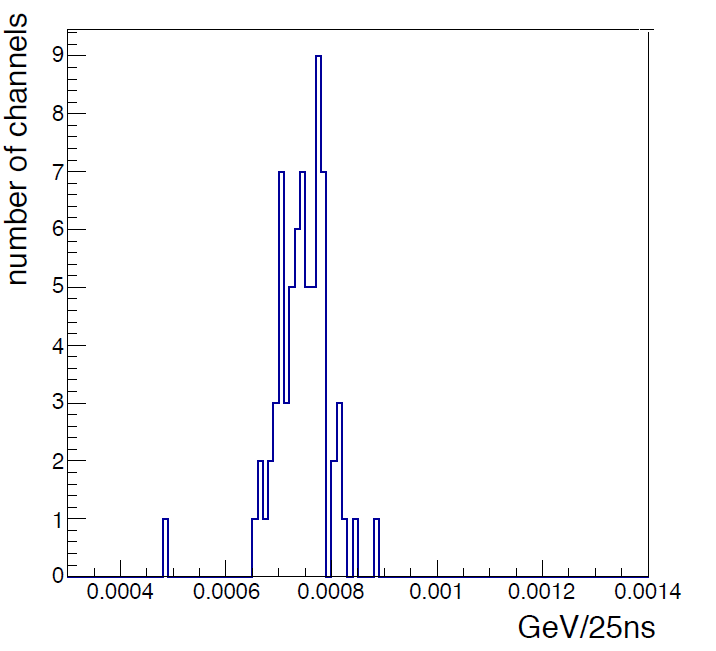
\includegraphics[width=.45\textwidth]{figures/ch_hfcalibration/HFM_2013_Res_EM.png}
      }~
      \subfigure[]{
         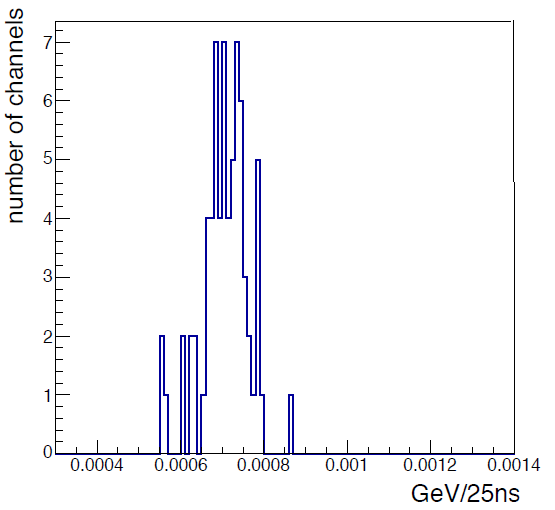
\includegraphics[width=.45\textwidth]{figures/ch_hfcalibration/HFM_2013_Res_H.png}
      }
      \caption{(a) EM Energy deposition for each tower below IEta = 35. (b) H Energy deposition for the same towers}
      \label{fig:HFM_2013_Res}
   \end{center}
\end{figure}

\subsection{2014 Results}
The source signals, ${\langle{Q}\rangle}^{Geom}_{c}$, for HF+ and HF- for 2014 data with new PMTs, corrected for geometry (geometry containment factor), firmware used (1TS or 2TS), Operating Voltage to be used (converting to OV2 from either OV1 or OV+100), are calculated using Eq.~\ref{eq:Sig_OV2} and are presented in Figure~\ref{fig:Signal_@OV2_TT0_withoutOF_FORDN}.
\begin{figure}[!h]
	\begin{center}
		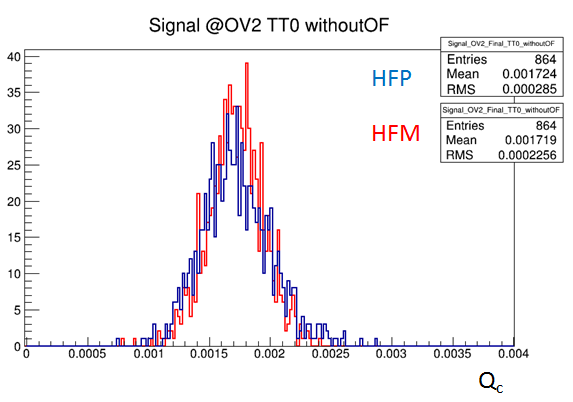
\includegraphics[width=.5\textwidth]{figures/ch_hfcalibration/Signal_@OV2_TT0_withoutOF_FORDN.png}
		\caption{Actual Signal from the Source recorded by the PMT @OV2 (Operational Voltage 2)}
		\label{fig:Signal_@OV2_TT0_withoutOF_FORDN}
	\end{center}
\end{figure}

The HF Gains, ${CC}^{Run II}_{c}$ in units of GeV/ADC, for HF+ and HF- are
computed using Eq.~\ref{eq:HF_Gains} and are presented in Figure~\ref{fig:ADC2GeV_OV2_TT0_withoutOF_FORDN}. In Eq.~\ref{eq:HF_Gains}, if $c$ is a EM channel form a given tower, then we use the EM result from 2013, and similar logic applies for the HAD channel
counterparts.
\begin{figure}[!h]
	\begin{center}
		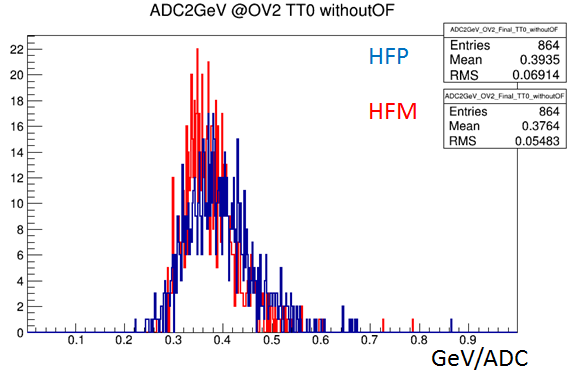
\includegraphics[width=.5\textwidth]{figures/ch_hfcalibration/ADC2GeV_OV2_TT0_withoutOF_FORDN.png}
		\caption{Distribution of Calibration Coefficients (HF Gains)}
		\label{fig:ADC2GeV_OV2_TT0_withoutOF_FORDN}
	\end{center}
\end{figure}

To account for the differences in Operating Voltages for Sourcing vs Run II Physics campaign, we applied the PMT Gain Ratios as Conversion Factors, distributions of which can be found in Figure~\ref{fig:PMT_Gains}
\begin{figure}[!h]
	\begin{center}
		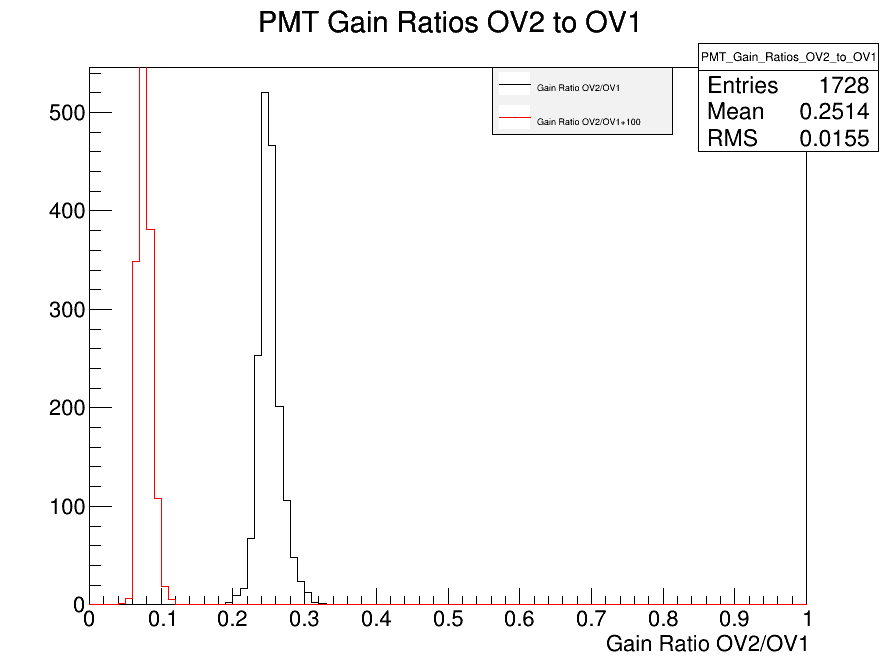
\includegraphics[width=.5\textwidth]{figures/ch_hfcalibration/GainRatios.png}
		\caption
		{Black - Ratio of PMT Gains for OV2/OV1; Red - Ratio of PMT Gains for OV2/OV1+100.
		}
		\label{fig:PMT_Gains}
	\end{center}
\end{figure}

\subsection{HF Gains and CondDB Submission}
To finalize the HF Source Calibration, we had to upload the computed calibration
coefficients, ${CC}^{Run II}_{c}$, into the Conditions DataBase (CondDB).
However, up until now, the units we used to present them were GeV/ADC, whereas
for submission it is required to provide calibration coefficients in GeV/fC.

\begin{figure}[htb]
	\begin{center}
		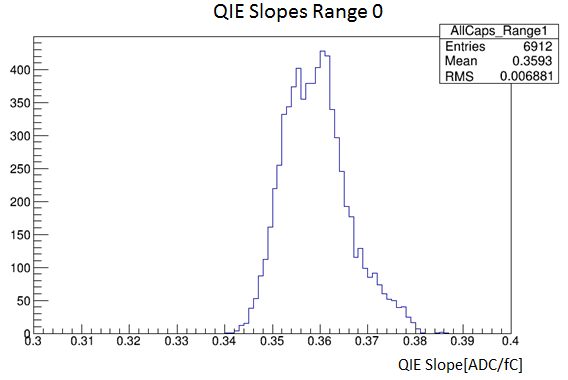
\includegraphics[width=.5\textwidth]{figures/ch_hfcalibration/QIE_Slopes_Range0.png}
		\caption{Distribution of Range 0 QIE Slopes}
		\label{fig:QIESlopes}
	\end{center}
\end{figure}

Therefore, we first extracted the ADC to fC conversion factors from the CondDB,
which are also called "QIE Slopes". As we have only been using Range 0 for
calibration purposes, they are the only ones of interest to us. At the time when
the actual analysis was performed, the half of the QIE Slopes were still mixed
up, as a consequence we averaged out all the slopes and used the mean for
converting our GeV/ADC to GeV/fC. In the Figure~\ref{fig:QIESlopes}, the
distribution of Range 0 QIE Slopes is presented. The obtained mean of 0.3593
(ADC/fC), as it was already pointed out, has been used to calculate the "final"
calibration coefficients in units of GeV/fC, which are presented in the
Figure().
Using the mean of Range 0 QIE Slopes adds an additional
uncertainty of 2\%, which can be deduced from the spread in the distribution of
QIE Slopes in the Figure~\ref{fig:QIESlopes}.

